\documentclass[12pt,a4paper,titlepage,twoside]{report}
\usepackage[utf8]{inputenc}
\usepackage[french]{babel}
\usepackage[T1]{fontenc}
\usepackage{amsmath}
\usepackage{amsfonts}
\usepackage{amssymb}
\usepackage{graphicx}
\usepackage{url}
\usepackage[usenames,dvipsnames]{xcolor}
\usepackage[colorlinks=false,urlbordercolor=white,linkbordercolor=white]{hyperref}
\usepackage[left=2cm,right=2cm,top=2cm,bottom=2cm]{geometry}
\usepackage{fancyhdr}
\usepackage{lmodern}
\usepackage{listings}
\pagestyle{fancy}
\usepackage{titlesec}
\usepackage[abs]{overpic}

% Definition des couleurs
\definecolor{titreColor}{RGB}{0,58,128}  % Marine
\definecolor{stitreColor}{RGB}{0,158,224}  % Ocean
\definecolor{auteurColor}{RGB}{0,58,128}     % Marine
\definecolor{texteColor}{RGB}{164,196,0}     % Prairie

% Definition des chapitres
\titleformat{\chapter}[display]
{\normalfont\Large\filcenter\sffamily}
{\titlerule[1pt]%
 \vspace{1pt}%
 \titlerule
 \vspace{1pc}%
 \Large\color{titreColor}{\MakeUppercase{\chaptertitlename} \thechapter}}
{1pc}
{\titlerule
 \vspace{1pc}%
 \Huge}

\titleformat{\section}
{\color{titreColor}\normalfont\Large\bfseries\sffamily}
{\color{titreColor}\thesection}{1em}{}

\titleformat{\subsection}
{\color{stitreColor}\bfseries\sffamily}
{\color{stitreColor}\thesubsection}{1em}{}

%Données de titre et d'auteur pour la page de garde
\newcommand{\titre}{Développement de l'application web USACT}
\newcommand{\sousTitre}{Stage de DUT Informatique réalisé par \newline Jérémy DAMEY \newline Du 7 avril au 12 juin 2015}
\newcommand{\auteur}{Jérémy DAMEY}
\newcommand{\dateModif}{\today}

\begin{document}
%Supprime les veuves et orphelines
\widowpenalty=10000
\clubpenalty=10000
\raggedbottom 

% Integre la page de garde
%\input{title.tex}
Maître de stage : Eric QUINTON \newline
Enseignant referent : Franck RUBI \newline
%\setcounter{page}{0}
\thispagestyle{empty}
\vspace*{7cm}
\setlength\unitlength{1mm}
% Logo de titre
\begin{overpic}[width=9.44cm,height=9.57cm,keepaspectratio]{Image/logo_fond.png}
% Titre du document
\put(30,50){
\begin{minipage}{0.7\linewidth}
\Huge\flushleft \color{titreColor}{\bfseries\sffamily\titre{}}\\
% sous-titre du document
\color{stitreColor}{\Large \bfseries\sffamily\sousTitre{}}
\end{minipage}
}
\end{overpic}

%  date et auteur
% creation de l'espace a gauche
\vspace*{1cm}
\begin{minipage}{0.5\linewidth}
\hfill
\end{minipage}
% positionnement
\begin{minipage}{0.5\linewidth}\flushleft{
% Date
\textcolor{auteurColor}{\Large\sffamily\dateModif{}}\\
\vspace*{0.1cm}
% Auteur
\textcolor{auteurColor}{\Large\sffamily\auteur{}}\\
\vspace{0.5cm}
% Adresse
\textcolor{texteColor}{\sffamily\textbf{IRSTEA} - Centre de Bordeaux\\
50, avenue de Verdun, Gazinet\\
33612 CESTAS Cedex }
}
\end{minipage}
% Ligne de logos
\begin{minipage}{\linewidth}
% Logo IRSTEA
\vspace{1.3cm}
\hspace{-1.4cm}

\includegraphics[width=3.06cm,height=9.57cm,keepaspectratio]{Image/logo_irstea}%
% logos complémentaires
\vspace{-1cm}
\hspace{2cm}
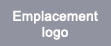
\includegraphics[width=3cm,height=3cm,keepaspectratio]
{Image/emplacement_logo}%
\vspace{-1cm}
\hspace{1cm}
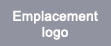
\includegraphics[width=3cm,height=3cm,keepaspectratio]
{Image/emplacement_logo}%
\vspace{-1cm}
\hspace{1cm}
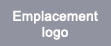
\includegraphics[width=3cm,height=3cm,keepaspectratio]
{Image/emplacement_logo}%
\end{minipage}
% Définition des entêtes
\fancyhead{}
\fancyhead[CO]{\leftmark\sffamily}
\fancyhead[CE]{ \sffamily\titre{}}
\fancyfoot[CO]{\sffamily\thepage}
\fancyfoot[CE]{\sffamily\thepage}
% Redéfinition de \cleardoublepage pour créer une page vide
\makeatletter
\def\cleardoublepage{\clearpage\if@twoside \ifodd\c@page\else
  \hbox{}
  \vspace*{\fill}

  \vspace{\fill}
  \thispagestyle{empty}
  \newpage
  \if@twocolumn\hbox{}\newpage\fi\fi\fi}
\makeatother

% \cleardoublepage permet de générer une page vide 
% si le chapitre ne commence pas sur la page de droite
\cleardoublepage
\vspace{1cm}
\begin{center}
\bf 
\color{titreColor}
\LARGE{Remerciements}
\end{center}
Tout d'abord, je tiens à remercier mon maître de stage Eric QUINTON pour m'avoir accepté au sein de l'IRSTEA et pour tout ce qu'il m'a apporté durant la durée de ce stage. \newline\newline
Je remercie également les chercheuses Sandrine LYSER et Clarisse CAZALS pour leurs disponibilités et les éclaircissements qu'elles m'ont apportés pendant ces 10 semaines. \newline\newline
Je tenais également à remercier l'IRSTEA pour l'accueil chaleureux que j'ai reçu. \newline\newline
Enfin, je remercie mes professeurs pour tout ce qu'ils m'ont apporté au cours de ces 2 années de formation. 

\setcounter{tocdepth}{4}
\tableofcontents
\cleardoublepage
\chapter{Présentation de l'IRSTEA}
\section{L'IRSTEA de manière général}
\section{L'IRSTEA à Bordeaux}
Le centre de recherche de Bordeaux est l’une des neuf implantations d'Irstea. Localisé sur le site principal de Cestas – Gazinet, ses activités de recherche, d’appui aux politiques publiques et d’expertise portent sur 2 domaines principaux : la gestion de l’eau et du fonctionnement des milieux aquatiques et l’interface entre eau et gestion des territoires. \newline\newline
Ses recherches sont effectuées en collaboration avec des laboratoires publics français ou européens (Université de Bordeaux, Université de Pau, CNRS, INRA ...) et des entreprises ou bureaux d’études privés. \newline\newline
Au sein du centre de Bordeaux, il y a deux unités de recherche :
\begin{description}
\item[- Ecosystèmes aquatiques et changements globaux (EABX) : ]Cette unité axe ses actions de recherche et d’expertise sur l’eau, sur la qualité des hydrosystèmes continentaux et sur l’appréciation de l’état et de la dynamique de fonctionnement des milieux et espèces susceptibles d’agir sur les édifices biologiques (pêche, perturbations, obstacles, contamination, changements environnementaux),
\item[- Environnement, territoires et infrastructures (ETBX) : ] Cette unité développe des recherches sur les dynamiques territoriales en lien avec le renouvellement des enjeux environnementaux et le changement climatique.
\end{description}
Ci-dessous, l'organigramme de l'unité ETBX (figure 1). J'ai intégré l'équipe EADT (Environnement, Acteurs et Dynamiques Territoriales). \newline
\clearpage
\begin{figure}
\center
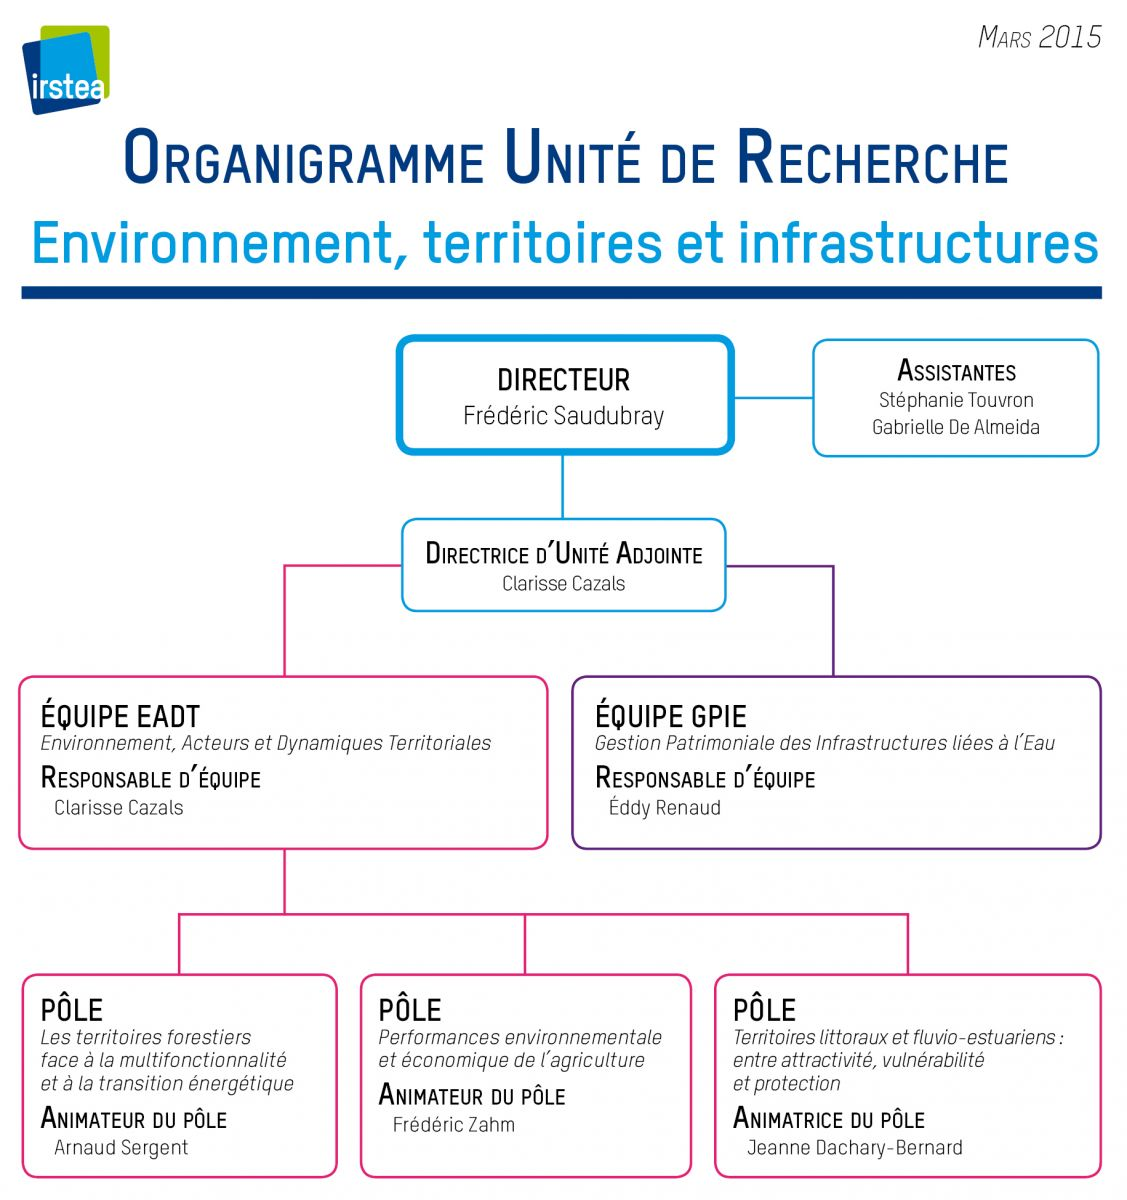
\includegraphics[width=12cm,height=15cm,keepaspectratio]{Image/Organigramme_UR_ETBX}%
\caption{Organigramme de l'unité ETBX} 
\end{figure}



\begin{tabbing}
Voici \= quelques chiffres sur les effectifs de Bordeaux : \\
\> - 2 unités de recherche \\
\> - 1 équipe services généraux et appui à la recherche \\
\> - 180 personnes dont la moitié de chercheurs et d'ingénieurs \\
\> - En moyenne 20 doctorants et post-doctorants par an \\
\> - Entre 30 et 35 agents en Contrat à Durée Déterminée \\
\> - Entre 25 et 30 stagiaires de l'enseignement supérieur \\
\> - 7 millions d'euros de budget annuel (hors salaires personnel permanent), dont 70 \% provenant \\ 
\> de ressources propres par contrats de recherche ou transferts. \newline\newline
\end{tabbing}

L'équipe EADT travaille sur la gestion des conflits au sein du basin d'Arcachon. Par la suite, nous allons voir les cas d'utilisations que j'ai établis avant de vraiment commencé la réalisation du projet. Ensuite nous verrons les nouveaux outils que j'ai utilisé et leur fonctionnement. Enfin, nous verrons à quoi ressemble le logiciel. 


% Second chapitre
\cleardoublepage
\chapter{Second chapitre}
% \input{chapitre2}

\end{document}
